\documentclass[]{article}
\usepackage{ txfonts  }
\usepackage{ graphicx  }


%opening
\title{Documentation on simulating RREA and RFD}
\author{Brian Hare}

\begin{document}

\maketitle

%\begin{abstract}

%\end{abstract}

\section{table of constants}

\begin{center}
	\begin{tabular}{ c c c }
		Name                            & symbol    &   value  \\ 
		speed of light                  & C         &         \\  
		charge of electron              & -e        &         \\  
		molecular density of air        & $N_m$     &   $2.688\times 10^{25} m^{-3} $     \\  
		average molecular charge of air & $Z_m$     &  14.5       \\  
		classical electron radius       & $r_e$     &   $2.8179\times 10^{-15} m $      \\  
        mass of electron                & $m_e$     &     \\
        ionization potential of ai  r   & $I$       &  85.7 ev    \\  
	\end{tabular}
\end{center}


\section{dimensionless variables}

Dimensionless variables are used in this simulation. This can complicate translating a physical equation into the simulation, but once in the simulation the formulas tend to be simpler. In the rest of this documentation, the normal symbols, e.g. $\varepsilon$ for kinetic energy and $ \vec{P} $ for momentum, will represent the values of those quantities in MKS units, alternate symbols will be used to represent the values of each quantity in dimensionless units, e.g. $E$ for kinetic energy and $\vec{\rho} $ for momentum. The table below gives the units of all the dimensionless variables used in the simulation. Brackets around a symbol, e.g.  $\left[ E\right] $ for energy and $\left[  \vec{\rho} \right] $ for momentum, represents the units of the dimensionless values, e.g. $\varepsilon = E \left[ E \right] $.

\begin{center}
	\begin{tabular}{ c c c }
		Name                 & units                             &   alternate symbol  \\ 
		time                 & $(2\pi N_m Z_m r^2_e C)^{-1}$     & $ \tau$    \\  
		velocity             & C                                 &  $\vec{\beta}$       \\  
		position             & $C\times \left[ \tau \right] $    & $ \vec{\chi} $     \\
		momentum             & $m_e C $                          &  $\vec{\rho} $     \\
		energy               & $m_e C^2 $                        &  E (kinetic only)      \\
		force                & $\frac{m_e C}{ \left[ \tau \right]} $     & $ \frac{d\vec{\rho}}{d\tau}$       \\
		electric field       & $\frac{m_e C}{ e \left[ \tau \right]} $   & $  \vec{\xi}  $   \\
		magnetic field       & $\frac{m_e }{ e \left[ \tau \right]} $    &  $ \vec{\Upsilon} $     \\
	\end{tabular}
\end{center}

\section{relativistic equations}

This simulation deals with very relativistic particles, and so must use relativistically correct formula. Since, in the simulation, each particle stores position and momentum, of particular interest is simple formula relating momentum to other quantities.

First, is the definition of gamma:
\begin{equation}
\gamma = \frac{1}{ \sqrt{1-\beta^2 } }
\end{equation}

Allowing us to define total energy:
\begin{equation}
\varepsilon_t = \gamma m_e C^2
\end{equation}

or in dimensionless units:

\begin{equation}
E_t = \gamma 
\end{equation}

The definition of kinetic energy:
\begin{equation}
\varepsilon_t = m_e C^2 + \varepsilon
\end{equation}

and in dimensionless units:
\begin{equation}
E_t = 1 + E
\end{equation}

Substitution gives us:
\begin{equation}
E=\gamma-1
\end{equation}

Next is the definition of momentum:

\begin{equation}
\vec{P} = \gamma m_e \vec{V}
\end{equation}

In dimensionless units:

\begin{equation}
\vec{\rho}= \gamma \vec{\beta}
\end{equation}

We can relate momentum to energy:
\begin{equation}
\varepsilon_t^2=(M_eC^2)^2 + (PC)^2
\end{equation}

dimensionless:
\begin{equation}
E_t^2=1+\rho^2
\end{equation}

Or:
\begin{equation}
\gamma^2=1+\rho^2
\end{equation}

thus:
\begin{equation}
E=\sqrt{1+\rho^2}-1
\end{equation}

Substitution gives:
\begin{equation}
\beta^2=\frac{\rho^2}{1+\rho^2}
\end{equation}


\section{forces and equations of motion}

The simplest task that needs to be done in the simulation is to simulate the motion of a particle given a electric field, magnetic field, and friction due to ionization.

In dimensionless units, the equations of motion for an electron are:

\begin{equation}
\frac{d \vec{\rho}}{ d \tau} = -\vec{\xi}(\vec{\chi}) -\frac{\vec{\rho} \times \vec{\Upsilon}(\vec{\chi}) }{\sqrt{ 1 + \rho^2 }} + \hat{\rho} \frac{d \rho}{d \tau}_{friction}(\rho)
\end{equation}

and 

\begin{equation}
\frac{d \vec{\chi}}{d \tau} = \frac{\vec{\rho}}{\sqrt{1+\rho^2}}
\end{equation}

Where $\frac{d \rho}{d \tau}_{friction}(\rho)$ is the friction force due to ionization. Since the frictional force can vary by multiple orders of magnitude over the energy range of interest, then we have to use a good adaptive solver for these equations. At this point in time the simulation is using the Cash-Karpe Runge Kutta technique. However, in the future we may want to consider using Doramund-Prince Runga Kunga, since it will give use one higher order with no extra cost and will allow for advanced interpolation of the particle's position and momentum in-between time steps. Presently we assume that the particle's position and momentum changes linearly between time steps. This is probably not very precise, but also probably doesn't actually introduce much error into the simulation. There is plenty of information on line about both pertinent Runga Kutta techniques.

The frictional force due to ionization could be approximated using the Bethe formula, this however, produces some problems as the Bethe formula is imprecise at low energies. Instead, we use tabulated values from ICRU report 37, which gives the energy loss due to ionization for electrons and positrons down to very low energies. The energy loss vs energy is re-sampled precisely in logarithmic space so that, in theory, the lookup time can be constant vs the size of the array. Finally, the table is then linearly interpolated in log-log space so that we can find approximate energy losses in between sample points. 

The tables in ICRU 37 extend to very high energy, and so probably will not need to generate new values using the Beth formula. However, this ability has been included should the need arise. (Note that we do not actually include the entire ICRU 37 table, it may be wise to extend the bit of the table that we do include).

Since we include M$\o$ller scattering in the simulation, the simulation takes M$\o$ller scattering into account by subtracting off the energy loss due to M$\o$ller scattering at the appropriate energies, given below, from Dwyer:


\begin{equation}
f_{m\o ller}=\frac{2\pi N_m Z_m r_e^2 m_e C^2}{\beta^2}\left[ ln\left( \frac{\varepsilon}{2K_{min}} \right) +1 - \frac{K_{min}}{\varepsilon- K_{min}} - \left(1+\frac{2}{\gamma}-\frac{1}{\gamma^2} \right) ln \left(   \frac{2(\varepsilon-K_{min})}{\varepsilon}\right) + \frac{(\gamma+1)^2}{8\gamma^2} - \frac{K_{min}^2}{2m_e^2C^4\gamma^2}   \right] 
\end{equation}

Where $\varepsilon$ is the kinetic energy of the electron, and $K_{min}$ is the minimum kinetic energy that we will produce new electrons from M$\o$ller scattering at. $K_{min}$ is adjustable and can be changed at the beginning of the simulation. we also technically include the ability to vary $K_{min}$ during the simulation, this ability however has not been tested.

In dimensionless units:

\begin{equation}
\frac{d \rho}{d \tau}_{m\o ller}=\frac{1}{\beta^2}\left[ ln\left( \frac{E}{2K_{min}} \right) +1 - \frac{K_{min}}{E- K_{min}} - \left(1+\frac{2}{\gamma}-\frac{1}{\gamma^2} \right) ln \left(   \frac{2(E-K_{min})}{E}\right) + \frac{E^2}{8\gamma^2} - \frac{K_{min}^2}{2\gamma^2}   \right] 
\end{equation}

Where $E$ is the kinetic energy of the electron in dimensionless units and $K_{min}$ is also dimensionless.

The Bethe equation (which approximates the frictional force due to ionization):

\begin{equation} 
F_{friction}(P)  =\frac{ 2 \pi N_m Z_m r_e^2 m C^2}{\beta^2} \left\lbrace  \ln\frac{mv^2\varepsilon\gamma}{I^2}
-\left( 1 + \frac{2}{\gamma}  - \frac{1}{\gamma^2} \right)\ln 2 + \frac{(\gamma-1)^2}{8\gamma^2}  + \frac{1}{\gamma^2} \right\rbrace 
\end{equation}

in dimensionless units:

\begin{equation} 
\frac{d \rho}{d \tau}_{friction}(\rho)  =\frac{ 1 }{\beta^2} \left\lbrace  \ln\frac{\beta^2E\gamma}{\bar{I^2}}
-\left( 1 + \frac{2}{\gamma}  - \frac{1}{\gamma^2} \right)\ln 2 + \frac{(\gamma-1)^2}{8\gamma^2}  + \frac{1}{\gamma^2} \right\rbrace 
\end{equation}

Where $\bar{I}$ is $I/m_eC^2$.

\section{Introduction to Discrete Events}

After we take one time step of length $\Delta \tau$ of the equations of motion, we then need to preform a number of discrete processes such as M$\o$ller and Bremsstrahlung scattering (and much more eventually). In order to preform these processes, we need to decide when and which process occurs. 

Each of these processes has a total cross section: $\sigma(E)$. We will index all the process by $i$, so that the $i^{th}$ process has the total cross section $\sigma_i(E)$. We relate each cross section to the rate of events by:

\begin{equation}
\frac{dn}{dt}_i = N V \sigma_i(E)
\end{equation}

With $\frac{dn}{dt}_i$ being the rate that the $i^{th}$ event occurs, N is the number density of targets, and V is the velocity.

In dimensionless units:

\begin{equation} \label{eq:CS_rate}
\frac{dn}{d\tau}_{i} = \frac{1}{2 \pi} \frac{N}{N_m} \beta \frac{\sigma_i(E)}{Z_mr_e^2}
\end{equation}

Which is more complicated, but actually tends to simplify many cross sections.

We can then add the rates together to get a total rate of discrete events:

\begin{equation}
\frac{dn}{d\tau}_{total} = \sum \frac{dn}{d\tau}_{i}
\end{equation}

We need to sample $\frac{dn}{d\tau}_{total}$ to find the time that an event occurs. Doing this to full numerical precision is rather difficult, since the energy, and thus the total rate of events, changes with time across the time step. So, instead, we assume that the rate of events changes linearly across the time step:

\begin{equation}
\frac{dn}{d\tau}_{total} = A + B\bar{T}
\end{equation}

Where $\bar{T}$ ranges from 0 at the beginning of the time step to 1 at the end. This method gives us control over the error, because the zeroth order error in this method is $\left| \frac{B}{A} \right| $. We have an $ \varepsilon_{low}$ (generally 0.1) and $ \varepsilon_{high}$ (generally 0.2) such that if the zeroeth order error exceeds $ \varepsilon_{low}$, then the next time step size is decreased by some factor (typically 2). and if the error exceeds  $ \varepsilon_{high}$, the the time step is completely re-done with a smaller step size (typically factor of 2). 

A and B are easily found:
\begin{equation}
A=\frac{dn}{d\tau}_{total}(\bar{T}=0)
\end{equation}

\begin{equation}
B=\frac{dn}{d\tau}_{total}(\bar{T}=1)-A
\end{equation}

Now we can find the time that some random event occurs by treating $\frac{dn}{d\tau}_{total}$ like a PDF and sampling it using inverse transform sampling (Google this term if it is not familiar, it is a staple technique that I use). 

First we integrate:
\begin{equation}
n(\bar{T})=\left( A\bar{T}+0.5B\bar{T}^2\right) \Delta \tau
\end{equation}

Normalize at $\bar{T}=1$ to find the CDF:
\begin{equation}
CDF(\bar{T})=\frac{\left( A\bar{T}+0.5B\bar{T}^2\right)}{n(\bar{T}=1)} \Delta \tau
\end{equation}

Invert to find $\bar{T}$ for some random number, $U$, uniform between 0 and 1 (Not 100 percent sure this next equation is correct, but not to worry, it is not actually used):

\begin{equation}
\bar{T}=-\frac{A}{B}  \pm  \sqrt{  \left( \frac{A}{B} \right)^2  + \frac{2Un(\bar{T}=1)}{B \Delta \tau }  }
\end{equation}

Where one would choose the solution between 0 and 1. This equation has a problem that it only gives the time of an event, assuming there is exactly one event. In order to use it properly, one needs to find $n(\bar{T}=1)$ (which is the average number of events in this time step). Sample the number of events that actually occurred from the Poisson distribution, then sample the above equation that many times and only keeping the lowest $\bar{T}$. All the other samples have to be thrown away, because if an event happens, then the event will likely change the energy of the particle, and so invalidate the following samples.

Instead, a better solution would be to find an equation that gives us the first $\bar{T}$ in a time step. To do this, we use the Poisson distribution to find the probability that there will be one or more events in the time from the start of the step to $\bar{T}$:

\begin{equation}
P(\bar{T})=1-\exp(-n(\bar{T}))=1.0-exp(-A\Delta \tau \bar{T} - 0.5B\Delta \tau\bar{T}^2)
\end{equation}

Solving for $\bar{T}$ gives us (where p is now a uniform random number between 0 and 1):

\begin{equation}
\bar{T}=-\frac{A}{B} \pm \sqrt{\left( \frac{A}{B} \right)^2 -\frac{2ln(1-p)}{B\Delta \tau} }
\end{equation}

Notice that if $B<0$, then there is a p where $\bar{T}$ is imaginary. Solving for this p gives us:

\begin{equation}
p_{max}=1-\frac{A^2\Delta \tau}{2B}
\end{equation}

If $B<0$ and $P>p_{max}$, then there is no event. Similarly if $\bar{T}>1$, then there is no event.

Also, if B is close to zero (much smaller than A), then the above equation becomes unstable. Instead we assume that the rate is constant with time. Solving for $\bar{T}$ gives us:

\begin{equation}
\bar{T}=-\frac{\exp(1-p)}{A\Delta \tau}
\end{equation}

Finally, we can decide which event happens by drawing a uniform random number, U, between 0 and 1. The $j^{th}$ event happens if:

\begin{equation}
\sum_{i=1}^{j}\frac{dn}{d\tau}_{i} < U\frac{dn}{d\tau}_{total} < \sum_{i=1}^{j+1}\frac{dn}{d\tau}_{i}
\end{equation}

NEEDS MORE WORK! Generic inverse transform sampling. Walker Aliased inverse transform sampling.

\section{Shielded Coulomb Scattering}

Note this this is not correct. There are too many factors of $Z_m$. See equation \ref{eq:CS_rate}.

As the electrons and positrons travel through the simulation, they will collide off of atomic nuclei. We simulate this by including the effects of elastic scattering off of atomic nuclei via the shielded coulomb cross section. The differential cross section for the shielded coulomb cross section is:

\begin{equation} 
\frac{d\sigma_{Coul}}{d \Omega} = \frac{1}{4}\left(  \frac{Z_m r_e }{\beta^2 \gamma }  \right)^2\frac{1-\beta^2\sin^2(\theta/2)}{ \left(  \sin^2(\theta/2) + \frac{\hbar}{4P^2a^2}  \right)^2 }
\end{equation}

where
\begin{equation} 
a=183.8 \lambdabar z_m^{-1/3}
\end{equation}

Using the definition of cross-sections, we can relate the differential cross section to expected number of times a particle will be deflected into an angle:

\begin{equation} 
\frac{dn}{d \Omega} =N_m Z_m V \Delta T \frac{d \sigma}{d \Omega}
\end{equation}

where $\frac{dn}{d \Omega}$ is the expected number of times that a particle will be deflected by angle $\Omega$ during time $\Delta T$. If $\frac{dn}{d \Omega} << 1$, it can be interpreted as a probability. 

In dimensionless units, this turns into:

\begin{equation} 
\label{dimensionless_cross_section_eq}
\frac{dn}{d \Omega} =\frac{ \beta \Delta \tau }{2 \pi r_e^2} \frac{d \sigma}{d \Omega}
\end{equation}

Plugging in the differential cross section for elastic shielded coulomb scattering gives:

\begin{equation}
\label{coulomb_scattering_rate_eq}
\frac{dn}{d \Omega} =\frac{ \Delta \tau }{8 \pi \beta }\left( \frac{Z_m}{\rho} \right)^2  \frac{1-\beta^2\sin^2(\theta/2)}{ \left(  \sin^2(\theta/2) + \frac{Z_m^{2/3}}{4\times 183.8^2} \frac{1}{\rho^2} \right)^2 }
\end{equation}

Two decisions need to be made using this formula. 1) How many times does a particle scatter in one time step, and 2) what angles does it scatter into? The first question can be answered by integrating equation \ref{coulomb_scattering_rate_eq} over the unit sphere for a given particle energy and time step, then by sampling the Poisson distribution. For shielded coulomb scattering, this turns out to be many many times for any reasonable time step. The second question is answered using inverse transform sampling. 

Inverse transform sampling is performed by first integrating the distribution over the relevant variable that needs to be sampled:

\begin{equation}
N(\theta) = \int_0^{\theta} sin(\theta ) d\theta '  \int_0^{2\pi} d\phi ' \frac{dn}{d\Omega}
\end{equation}

Normalizing and inverting the function such that:

\begin{equation}
N'\left(  \frac{N(\theta)}{N(\pi)}  \right) = \theta
\end{equation}

Then we can then sample a number between 0 to 1, from the uniform distribution, $U$, and plug it into $N'$ to get a sample for our variable:

\begin{equation}
N'\left(  U  \right) = \theta
\end{equation}

Except for a few specific cases, inverse transform sampling cannot be done analytically. I will describe a method I have developed to do inverse transform sampling reliably. After sampling the inclination, the azimuth, $\phi$ can be sampled from the uniform distribution. 

After the inclination and azimuth have been sampled, we can rotate the momentum vector by finding an orthogonal, but not normal, vector basis in which the momentum is one axis. First, we use cross products to find two vectors, $\vec{Bv}$ and $\vec{Cv}$ orthogonal to each other, and orthogonal to the momentum vector, $\vec{\rho}$:

\begin{equation}
\label{Bv_def}
\vec{Bv}=\frac{\vec{\varsigma}\times \vec{\rho}}{ \left| \vec{\varsigma}\times \vec{\rho}  \right|   }
\end{equation}

Where $\vec{\varsigma}$ is any unit vector chosen so that equation \ref{Bv_def} is not singular.

\begin{equation}
\vec{Cv}=\vec{Bv}\times \vec{\rho}
\end{equation}

$\vec{Cv}$ is guaranteed to have the same magnitude as the momentum, since $\vec{Bv}$ is guaranteed to be a unit vector orthogonal to the momentum.

Using these new basis vectors, we can calculate the new momentum:

\begin{equation}
\vec{\rho}_{new}= cos(\theta) \vec{\rho} + sin(\theta) cos(\phi) \vec{Bv} \left|\vec{\rho} \right| - sin(\theta) sin(\phi) \vec{Cv} 
\end{equation}

This process needs to be ran however many times scattering happened to occur for that time step. This process is very slow. So what is done, is that this process is ran many many times before the simulation, and a distribution for $\theta$ is built up for different energies and time steps. This distribution is then saved in a table and can be opened and sampled relatively quickly at simulation time.


\section{numerical inverse transform sampling}

My method for inverse transform sampling relies upon quadratic interpolation. We need a quadratic interpolant:

\begin{equation}
\label{second_order_interpolant_eq}
\bar{Y}(x)=W_1 +W_2 x + W_3 x^2
\end{equation}

Such that $\bar{Y}$ is precise at three points:

\[ \bar{Y}(X_L)=Y_L \]
\[ \bar{Y}(X_M)=Y_M \]
\[ \bar{Y}(X_R)=Y_R \]

Solving the 3x3 matrix reveals:

\begin{equation}
W_3=\frac{(X_M-X_L)(Y_R-Y_L) - (X_R-X_L)(Y_M-Y_L)  }{ (X_M-X_L)(X_R^2-X_L^2) - (X_R-X_L)(X_M^2-X_L^2)   }
\end{equation}

\begin{equation}
W_2=\frac{  Y_M - Y_L  }{ X_M-X_L  } - W_3 \frac{X_M^2-X_L^2}{X_M-X_L}
\end{equation}

\begin{equation}
W_1=Y_L - W_2X_L - W_3X_L^2
\end{equation}

Integrating this interpolant gives us an approximation for the cumulative integral of our function;

\begin{equation}
\label{quadrature_eq}
\int_{X_L}^{x} Y(x') dx' \approx \int_{X_L}^{x} \bar{Y}(x') dx' = W_1x + \frac{W_2}{2}x^2 + \frac{W_3}{3}x^3 -(W_1X_L + \frac{W_2}{2}X_L^2 + \frac{W_3}{3}X_L^3)
\end{equation}

Using this integral over multiple regions, we can have a method adaptive cumulative quadrature. This is done by first splitting the region we want to integrate over into multiple sections (say, 5). We then sample the function we want to integrate at the endpoints and at the middle of each section and estimate the area of each section using equation \ref{quadrature_eq}. We then split each section into a left and right subsections, and sample the function at the center of each subsection to get a slightly better estimate of the area.  Finally we test our precision using equation \ref{quadrature_condition_eq} below. Where $float(x)$ is the floating point representation of x. $A_s$, $A_l$, and $A_r$ are the areas of some section and its left and right subsections, and $F$ is a factor that controls our precision. 

\begin{equation}
\label{quadrature_condition_eq}
float(F*A_s + (A_s - A_l - A_r)) == float(F*A_s)
\end{equation}

For any subsection, if this condition is true, then we are done and move onto the next section. If this condition is not true then the two subsections are each split into two subsections and this procedure is repeated until condition \ref{quadrature_condition_eq} is true. In this way we can very precisely sample the integral of any function at a number of un-equally spaced points. I am not sure how this method will behave if the value of the integral is at or close to zero. I am using low-order polynomial quadrature instead of a more advance method, say a high-order Gaussian quadrature, because this method is relatively simple and easily produced a cumulative integral.

Finally, this cumulative integral is normalized and is inverted by plugging the value of the integral at each point into our interpolant (equation \ref{second_order_interpolant_eq}) for the x values and the points that the integral was sampled at for the y-values. We can then sample our distribution by sampling a variable from the uniform distribution and plugging that number into this inverse interpolant. This method can only sample one-dimensional distributions, but multi-dimensional distributions can always be turned into multiple one-dimensional distributions via integration.

\section{M\o ller scattering}

We need to include the production of multiple electrons via M\o ller scattering. Dwyer gives the cross section (in normal SI units) as:

\begin{equation} 
\frac{d\sigma_{M\o ller}}{d K} = \frac{2\pi r_e^2 m c^2}{\beta^2}\left[  \frac{(\gamma-1)^2m^2c^4}{K^2(mc^2(\gamma-1)-K)^2} - \frac{2\gamma^2 + 2\gamma -1}{K(mc^2(\gamma-1)-K)\gamma^2}  + \frac{1}{m^2c^4\gamma^2}  \right]
\end{equation}

Where K is the kinetic energy of the produced electron.

Plugging into equation \ref{dimensionless_cross_section_eq}, converting to dimensionless units, and doing some conversions gives:

\begin{equation} 
\label{dimensionless_moller_scattering_eq}
\frac{dn_{M\o ller}}{d E'} = \frac{\Delta \tau}{\beta}\left[  \frac{E^2}{E'^2(E-E')^2} - \frac{2\gamma^2 + 2\gamma -1}{E'(E-E')\gamma^2}  + \frac{1}{\gamma^2}  \right]
\end{equation}

(Note that, unlike shielded coulomb scattering above, this equation is actually somewhat correct in reference to eq \ref{eq:CS_rate}. Need to just turn delta tau into dtau and move to LHS)

Where E' is the dimensionless version of K, and E is the kinetic energy of the original electron before scattering. This equation can be turned into a distribution using the method discussed above for a number of pertinent energies, and these distributions can be saved in a table for later use. The normalization factor (used to normalize the distribution) will need to be saved as well in order to know how many times to sample the distributions.

In the main simulation, once equation \ref{dimensionless_moller_scattering_eq}, we need to use the final energy to find the angles of the two electrons.

\begin{figure}
\centering
\includegraphics[width=0.7\linewidth]{./figures/moller_kinematics/scattering_kinematics}
\caption{Diagram showing an electron scattering off of an electron at rest.}
\label{scattering_kin_fig}
\end{figure}

Figure \ref{scattering_kin_fig} shows an electron scattering off an electron at read. We know the initial energies of the two electrons, we know the final energy of the new electron, F2, as this was sampled from equation \ref{dimensionless_moller_scattering_eq}, so using conservation of energy we know the energy of the final electron F1 as well. We need to use relativistic kinematics to find than angles $\theta_1$ and $\theta_2$. We start with energy/momentum conservation, where the tilde means that the momentum is a 4-vector:

\[ 
\tilde{P_{I1}}+\tilde{P_{I2}}=\tilde{P_{F1}}+\tilde{P_{F2}}
\]

Moving and squaring:

\[ 
(\tilde{P_{I1}}-\tilde{P_{F1}})^2=(\tilde{P_{F2}}-\tilde{P_{I2}})^2
\]

Writing out the squares:

\[ 
\tilde{P_{I1}}^2 + \tilde{P_{F1}}^2 - 2\tilde{P_{F1}}\tilde{P_{I1}}=\tilde{P_{I2}}^2 + \tilde{P_{F2}}^2 - 2\tilde{P_{F2}}\tilde{P_{I2}}
\]

Using the fact that I2 is at rest and that any four-momentum squared is just the rest energy of the electron:

\[ 
2\varepsilon_r^2 - 2(\varepsilon_{I1}\varepsilon_{F1}- \vec{P_{I1}}\cdot\vec{P_{F1}})=2\varepsilon_r^2 - 2(\varepsilon_{F2}\varepsilon_r)
\] 

Where $\varepsilon$ is the total energy of the associated electron, and $\varepsilon_r$ is the rest energy of the electron. Solving for the dot product gives:

\[ 
cos(\theta_1)=\frac{\varepsilon_{I1}\varepsilon_{F1}-\varepsilon_{F2}\varepsilon_r}{ \left| \vec{P_{I1}} \right| \left| \vec{P_{F1}} \right|  }
 \]
 
In dimensionless units:

\begin{equation}
cos(\theta_1)=\frac{(E_{I1}+1)(E_{F1}+1)-(E_{F2}+1)}{\rho_{I1}\rho_{F1}}
\end{equation}

Similarly:

\begin{equation}
cos(\theta_2)=\frac{(E_{I1}+1)(E_{F2}+1)-(E_{F1}+1)}{\rho_{I1}\rho_{F2}}
\end{equation}

Where $E$ is the dimensionless kinetic energy of the associated particle and $\rho$ is the dimensionless momentum.

\end{document}
